\documentclass{article}
% if you need to pass options to natbib, use, e.g.:
%     \PassOptionsToPackage{numbers, compress}{natbib}
% before loading neurips_2020
% ready for submission
% \usepackage{neurips_2020}
% to compile a preprint version, e.g., for submission to arXiv, add add the
% [preprint] option:
%     \usepackage[preprint]{neurips_2020}
% to compile a camera-ready version, add the [final] option, e.g.:
     \usepackage[final]{neurips_2020}
% to avoid loading the natbib package, add option nonatbib:
%     \usepackage[nonatbib]{neurips_2020}
\usepackage[utf8]{inputenc} % allow utf-8 input
\usepackage[T1]{fontenc}    % use 8-bit T1 fonts
%\usepackage{hyperref}       % hyperlinks
\usepackage{url}            % simple URL typesetting
\usepackage{booktabs}       % professional-quality tables
\usepackage{amsfonts}       % blackboard math symbols
\usepackage{nicefrac}       % compact symbols for 1/2, etc.
\usepackage{microtype}      % microtypography
\usepackage{tikz}
\usepackage{amssymb}
\usepackage{amsthm}
\usepackage{amsmath}
\usepackage{mathabx}
\usepackage{natbib}
\usepackage{listings}
\usepackage{bbm}
\usepackage{caption}
\usepackage{float}
\usepackage{setspace}
\usetikzlibrary{patterns}
\def\E{\mathbb E}
\def\H{\mathcal H}
\def\R{\mathbb R}
\def\bfx{\mathbf x}
\def\argmax{\mathrm{argmax}}
\def\argmin{\mathrm{argmin}}
\def\sgn{\mathrm{sgn}}
\newcommand{\comment}[1]{\textcolor{red}{#1}}
\title{Incentive Incompatibility of Logistic Regression}
% The \author macro works with any number of authors. There are two commands
% used to separate the names and addresses of multiple authors: \And and \AND.
%
% Using \And between authors leaves it to LaTeX to determine where to break the
% lines. Using \AND forces a line break at that point. So, if LaTeX puts 3 of 4
% authors names on the first line, and the last on the second line, try using
% \AND instead of \And before the third author name.
\author{}
\begin{document}
\newtheorem{thm}{Theorem}
\newtheorem{cor}{Corollary}
\newtheorem{lem}{Lemma}
\newtheorem{prop}{Proposition}
\newtheorem{conj}{Conjecture}
\newtheorem{algo}{Algorithm}
\newtheorem{obs}{Observation}
\newtheorem{clm}{Claim}
\theoremstyle{definition}
\newtheorem{df}{Definition}
\newtheorem{eg}{Example}
\newtheorem{asm}{Assumption}
\newtheorem{cond}{Condition}
\theoremstyle{remark}
\newtheorem{rmk}{Remark}
\maketitle \allowdisplaybreaks \raggedbottom
\begin{abstract}
We study the incentive compatibility of multi-class logistic regression. We provide a numerical example in which a strategic data provider has the incentive to misreport her private label to increase the classification probability of her true label. In particular, the model trained given her true label classifies her data point incorrectly, whereas the model trained given her misreported label classifies her data point correctly. We show that this incentive incompatibility disappears for classifiers that satisfy a monotonicity condition and independence of irrelevant alternatives condition. Examples of such classifiers include Bayes classifiers, kernel density estimators, and empirical risk minimization classifiers with zero-one loss.
\newline \newline

\end{abstract}
























\section{Introduction} 
Consider an insurance company that makes its pricing decisions based on the customers' public observable characteristics, but the decision models are built using the information on private unobservable characteristics the customers' report. If the insurance company is transparent about its models, they might worry that customers have incentives to misreport their private information to get the contract that is the most beneficial to them. Similar examples include other rating systems that depend on the report of private information, such as loan applications, school grades, and employee screening.
\newline \newline
In a general mechanism design problem, each of many strategic agents owns one public data point and reports her private label to the principal. The principal is the learner and builds a classifier based on the labels provided by the agents. Each agent chooses a label to report, not necessarily her true label, to maximize the probability that her data point is classified correctly by the principal. We say that a dataset is incentive-incompatible for the classifier if at least one of the agents has the incentive to misreport, and we characterize classifiers that are incentive-compatible with all possible datasets.
\newline \newline
We start with an example dataset that is incentive-incompatible for the multi-class logistic regression classifier. In the dataset, each of the $18$ agents owns a two-dimensional data point and a private label with one of three values: "red", "green", or "blue".
\newline \newline

\begin{figure}[H] \centering 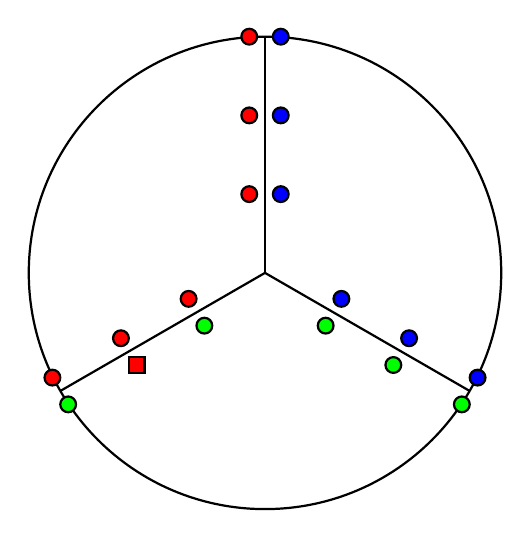
\begin{tikzpicture} [scale = 1] 
\draw[thick] (0.0, 0.0) circle [radius = 3.0];
\draw[thick] (0.0, 0.0) -- (0.0, 3.0);
\draw[fill = blue, thick] (0.2, 1.0) circle [radius = 0.1];
\draw[fill = blue, thick] (0.2, 2.0) circle [radius = 0.1];
\draw[fill = blue, thick] (0.2, 3.0) circle [radius = 0.1];
\draw[fill = red, thick] (-0.2, 1.0) circle [radius = 0.1];
\draw[fill = red, thick] (-0.2, 2.0) circle [radius = 0.1];
\draw[fill = red, thick] (-0.2, 3.0) circle [radius = 0.1];
\draw[thick] (0.0, 0.0) -- (2.6, -1.5);
\draw[fill = blue, thick] (0.97, -0.33) circle [radius = 0.1];
\draw[fill = blue, thick] (1.83, -0.83) circle [radius = 0.1];
\draw[fill = blue, thick] (2.7, -1.33) circle [radius = 0.1];
\draw[fill = green, thick] (0.77, -0.67) circle [radius = 0.1];
\draw[fill = green, thick] (1.63, -1.17) circle [radius = 0.1];
\draw[fill = green, thick] (2.5, -1.67) circle [radius = 0.1];
\draw[thick] (0.0, 0.0) -- (-2.6, -1.5);
\draw[fill = red, thick] (-0.97, -0.33) circle [radius = 0.1];
\draw[fill = red, thick] (-1.83, -0.83) circle [radius = 0.1];
\draw[fill = red, thick] (-2.7, -1.33) circle [radius = 0.1];
\draw[fill = green, thick] (-0.77, -0.67) circle [radius = 0.1];
\draw[fill = red, thick] (-1.73, -1.27) rectangle (-1.53, -1.07);
\draw[fill = green, thick] (-2.5, -1.67) circle [radius = 0.1];
\end{tikzpicture} \captionof{figure}{Incentive-incompatible Example}\label{fig:ice}
\end{figure}
The $18$ points are located inside a unit circle, and each point is $0.004$ away from the three line segments through the origin that forms angles of $120$ degrees between them. There is one red point, drawn as a square in the diagram, that is on the "incorrect" side of the boundary. For the agent represented by the red square, truthfully reporting her label will lead to a multi-class logistic regression model that classifies her point as "green". The probability that this model classifies her point as "red" is $0.3290$. However, if the agent misreports her label as "blue", the resulting model classifies her point as "red", and with a probability of $0.4966$. By lying about her label, the agent can make the principal learn an incorrect model that classifies her point correctly and with a higher probability.
\newline \newline
The example provides insight into the general incentive incompatibility issue of many classification models used in machine learning. The "red" agent that gets incorrectly classified as "green", does not want to misreport her label as "green" but instead has the incentive to misreport her label as the third alternative "blue" to influence the classifier in a way that changes the decision between "red" and "green". Intuitively, if there are only two classes, then the agent would not be willing to misreport her label if the classifier is monotonic, in the sense that adding a point from one class increases the probability that this point is classified as a member of that class; and if there are more than two classes, then the agent would not be willing to misreport her label if the classifier is independent of irrelevant alternatives, in the sense that adding a point from a third class would not affect the decisions between the two classes.
\newline \newline
Previous work on mechanism design for machine learning with strategic data sources focuses on designing robust algorithms to incentivize the data providers to report their private data truthfully. Their models mainly differ in the objective and the possible actions of the data providers (agents) and the learner (principal).
\newline \newline
The first group of papers focuses on principal-agent problems similar to our paper in which each agent's private data point is the agent's type that the agent cannot change. The only action the agents can take is whether to report their private information truthfully.
\begin{enumerate}
\item Some models assume the agents' data points (or feature vectors) are public, but their labels are private. \citet*{perote2004strategy}, \citet*{chen2018strategyproof}, and \citet*{gast2013linear} focus on strategy-proof linear regression algorithms and introduced clockwise repeated median estimators, generalized resistant hyperplane estimators, and modified generalized linear squares estimators. \citet*{dekel2010incentive} investigates the general regression problem with empirical risk minimization and absolute value loss. All the previously mentioned papers assume the labels are continuous variables (regression problems), and \citet*{meir2012algorithms} assumes the labels are discrete variables (classification problems) and proposes a class of random dictator mechanisms.
\item Some models assume the agents' data points are also private. \citet*{chen2019grinding} investigates such problems for linear regressions.
\item Other models do not involve labels. Each agent has a private valuation. These problems are usually modeled as facility location problems and the solution involves some variant of the Vickrey-Clarke-Groves or Meyerson auction. They include \citet*{dutting2017optimal}, \citet*{golowich2018deep}, \citet*{epasto2018incentive}, and \citet*{procaccia2009approximate}.
\end{enumerate}


The second group papers focus on moral-hazard problems in which each agent does not have a type but they can choose an action (with a cost) that affects the probability of obtaining the correct label. \citet*{richardsonprivately} focuses on the linear regression problem in this scenario, and \citet*{cai2015optimum} and \citet*{shah2016double} investigates the problem for more general machine learning problems. \citet*{mihailescu2010strategy} also discusses a similar problem for general machine learning algorithms.
\newline \newline
The last group of papers uses machine learning or robust statistics techniques without game-theoretic models. This group of papers include \citet*{dekel2009vox}, \citet*{dekel2009good}.
\newline \newline



\section{Logistic Regression} 

\subsection{Model}
In this section, we introduce the model using logistic regression as an example. We assume the principal is training a multi-class logistic (softmax) regression. There are $n $ strategic agents each providing the label of one data point to the principal. An agent, $i $, with public $x_{i} \in \mathbb{R}^{m}$, and private discrete $y_{i} \in \left\{1, 2, ..., k \right\}$, has the objective of maximizing the probability that her data point is labeled correctly by the principal's classifier, parameterized by the $m  \times \left(k  + 1\right)$ weights (and bias) matrix $w $. The agent can choose to report $y^{\dagger}_{i}$ to achieve the objective, with possibly $y^{\dagger}_{i} \neq  y_{i}$. Denoting the weights of the model resulting from the false report from agent $i $ by $w^\star \left(y^{\dagger}_{i}\right)$ (and $w^{\dagger}$ when the identity and the report of the agent is unambiguous), the agent's objective can be written as,
\begin{align*}
&  \displaystyle\max_{y^{\dagger} \in \left\{1, 2, ..., k \right\}} \mathbb{P}\left\{Y = y_{i} | x_{i} ; w^\star \left(y^{\dagger}_{i}\right)\right\},
\end{align*}
where,
\begin{align*}
&  \mathbb{P}\left\{Y = c | x_{i} ; w\right\} = \dfrac{e^{z_{i,c}}}{\displaystyle\sum_{c'=1}^{k} e^{z_{i,c'}}},
\\ &  z_{i,c} = \displaystyle\sum_{j=1}^{m} w_{j,c} x_{i,j} + b_{c} , \text{\;for\;} c \in \left\{1, 2, ..., k\right\}.
\end{align*}
The principal is not strategic and he maximizes the likelihood of the data,
\begin{align*}
&\displaystyle\max_{w} \displaystyle\sum_{i=1}^{n} \log\left(\mathbb{P}\left\{Y = y^{\dagger}_{i} | x_{i} ; w\right\}\right).
\end{align*}
We consider the case without a coalition of a group of agents, so only one agent is misreporting at a time, and use the following notations,
\begin{align*}
w^\star  &= \arg\displaystyle\max_{w} \displaystyle\sum_{i=1}^{n} \log\left(\mathbb{P}\left\{Y = y_{i} | x_{i}; w\right\}\right), \text{\;and\;}
\\ w^{\dagger} &= w^\star \left(y^{\dagger}_{i}\right) = \arg\displaystyle\max_{w} \log\left(\mathbb{P}\left\{Y = y^{\dagger}_{i} | x_{i}; w\right) + \displaystyle\sum_{i' = 0, i' \neq  i}^{n} \log\left(\mathbb{P}\left\{Y = y_{i'} | x_{i'}; w\right\}\right).\right.
\end{align*}
\begin{df} \label{df:ic} 
A dataset is incentive-incompatible for a classifier if there exists at least one agent $i $, and some $y^{\dagger}_{i} \neq  y_{i}$ such that,
\begin{align*}
\mathbb{P}\left\{Y = y_{i} | x_{i}; w^\star \right\} &< \mathbb{P}\left\{Y = y_{i} | x_{i}; w^\star \left(y^{\dagger}_{i}\right)\right\}.
\end{align*}
A classifier is incentive-compatible if there does not exist a dataset that is incentive-incompatible for the classifier.
\newline \newline\end{df}
\begin{conj} \label{conj:logit} 
Multi-class logistic regression is not incentive-compatible.
\newline \newline\end{conj}
The example described in Figure \ref{fig:ice} is a dataset that is numerically incentive-incompatible.
\\* In this example, agent $i $ reports $x_{i} \in \mathbb{R}^{2}$ and $y_{i}$ is one of $1$ (red), $2$ (green), or $3$ (blue). Suppose the red square point corresponds to agent $1$ with $x_{1} = \left(-1.63, -1.17\right)$ and $y_{1} = 1$, then
\begin{align*}
\mathbb{P}\left\{Y = 1 | x_{1} ; w^\star \right\} &= 0.3290,
\\ \mathbb{P}\left\{Y = 1 | x_{1} ; w^\star \left(y^{\dagger}_{1} = 3\right)\right\} &= 0.4966.
\end{align*}
Here, parameter estimation is done using maximum likelihood estimation with BFGS, and $w^\star $ is given by, with class $1$ weights normalized to $0$,

\begin{center} \begin{tabular}{|c|c|c|c|c|}
\hline
 Class &(Intercept) &x1 &x2\\ \hline
$1$ &$0$ &$0$ &$0$\\ \hline
$2$ &-$0.6053178$ &$104.9925$ &-$181.3391914$\\ \hline
$3$ &-$0.2852057$ &$209.4190$ &$0.3656777$\\ \hline
\end{tabular} \end{center}
and $w^\star \left(y^{\dagger}_{1} = 3\right)$ is given by,

\begin{center} \begin{tabular}{|c|c|c|c|c|}
\hline
 Class &(Intercept) &x1 &x2\\ \hline
$1$ &$0$ &$0$ &$0$\\ \hline
$2$ &-$0.1915645$ &$3.473426$ &-$5.507418$\\ \hline
$3$ &$0.8273350$ &$4.309293$ &-$1.200060$\\ \hline
\end{tabular} \end{center}
Currently, there is no formal proof that the result is not due to numerical instability, therefore, @(logit) is stated as a conjecture. Numerical experiments indicate that incentive-incompatible datasets are rare. If the data points are two-dimensional and standard normally distributed, and the labels are created using randomly generated weights with a small probability of error, then such a dataset is incentive-incompatible with a probability of $0.005$.
\newline \newline


\subsection{Loss Functions}
It is, however, possible to change the loss function so that logistic regression is incentive-compatible. Changing the loss function to absolute value $L^{1}$ loss is one possibility, due to \citet*{dekel2010incentive}. Their result on incentive compatibility of empirical risk minimization in the regression setting is applicable in our model. In addition to absolute value loss, empirical risk minimizers with zero-one loss are also always incentive-compatible.
\newline \newline
\begin{prop} \label{prop:zolog} 
Multi-class deterministic empirical risk minimization classifiers with zero-one loss are incentive-compatible.
\end{prop}
\begin{proof} \label{proof:zologpf} 
For any dataset $\left\{\left(x_{i}, y_{i}\right)\right\}_{i=1}^{n}$, and the hypothesis class $\mathcal{H}$, let the optimal classifier be,
\begin{align*}
h^\star  &= \arg\displaystyle\min_{h \in \mathcal{H}} \displaystyle\sum_{i'=1}^{n} \mathbbm{1}_{\left\{y_{i'} \neq  h\left(x_{i'}\right)\right\}}.
\end{align*}
Fix an agent $i $ with $x_{i}$, and fix the other agents' reports, $\left(x_{-i}, y_{-i}\right)$, define the loss function given the classifier $h $ and report of agent $i , y^{\dagger}_{i}$, as,
\begin{align*}
\ell\left(y^{\dagger}_{i}; h\right) &= \displaystyle\sum_{i' \neq  i} \mathbbm{1}_{\left\{y_{i'} \neq  h\left(x_{i'}\right)\right\}} + \mathbbm{1}_{\left\{y^{\dagger}_{i} \neq  h\left(x_{i}\right)\right\}}.
\end{align*}
If $y_{i} = h^\star \left(x_{i}\right)$, then the classifier is already classifying $x_{i}$ correctly, misreporting will not improve the outcome for $i $. Assume the prediction is $h^\star \left(x_{i}\right) = y^\star  \neq  y_{i}$, and suppose $h^\star $ is making $q $ mistakes, meaning,
\begin{align*}
q  &= \displaystyle\min_{h \in \mathcal{H}} \ell\left(y_{i} ; h^\star \right).
\end{align*}
Agent $i $ can misreport in the following two ways:
\end{proof}
\begin{enumerate}
\item If agent $i $ reports $y^{\dagger}_{i} = y^\star $, let the new classifier be $h^{\dagger}$, note that we must have,
\begin{align*}
\ell\left(y^\star  ; h^{\dagger}\right) &\leq  q - 1,
\end{align*}
since $\ell\left(y^\star  ; h^{\dagger}\right) > q - 1 = \ell\left(y^\star  ; h^\star \right)$ contradicts the optimality of $h^{\dagger.}$
\\* Suppose that agent $i $ could get her true label with $h^{\dagger}$, meaning $h^{\dagger}\left(x_{i}\right) = y_{i}$, then,
\begin{align*}
\ell\left(y_{i} ; h^{\dagger}\right) &= \ell\left(y^\star  ; h^{\dagger}\right) - 1
\\ &\leq  k - 2
\\ &< \ell\left(y_{i} ; h^\star \right),
\end{align*}
which contradicts the optimality of $h^\star $. Therefore, agent $i $ cannot improve the outcome by misreporting $y^\star $.
\item If agent $i $ reports $y^{\dagger}_{i} = y' \neq  y^\star $, let the new classifier be $h^{\dagger}$, note that we must have,
\begin{align*}
\ell\left(y' ; h^{\dagger}\right) &\leq  q,
\end{align*}
since $\ell\left(y' ; h^{\dagger}\right) > q = \ell\left(y' ; h^\star \right)$ contradicts the optimality of $h^{\dagger.}$
\\* Suppose that agent $i $ could get her true label with $h^{\dagger}$, then,
\begin{align*}
\ell\left(y_{i} ; h^{\dagger}\right) &= \ell\left(y_{i} ; h^{\dagger}\right) - 1
\\ &\leq  q - 1
\\ &< \ell\left(y_{i} ; h^\star \right),
\end{align*}
which contradicts the optimality of $h^\star $. Therefore, agent $i $ cannot improve the outcome by misreporting $y'$.
\\* Therefore, no agent can improve the outcome and the dataset is incentive-compatible.
\newline \newline
\end{enumerate}


\subsection{Binary Logistic Regression}
Binary logistic regression is always incentive-compatible, and agents with one label do not want to pretend to have the other label. This is not true in general for binary empirical risk minimization classifiers, and additional normalization condition on the loss function is required. The result is discussed in the next section. In the special case of logistic regression, since $\ell\left(0 ; h\right) + \ell\left(1 ; h\right) = 1$ holds for any $h  \in \mathcal{H}$, the following Proposition holds.
\newline \newline
\begin{prop} \label{prop:bin} 
Binary logistic classifiers are incentive-compatible.
\end{prop}
\begin{proof} \label{proof:binpf} 
For any dataset $\left\{\left(x_{i}, y_{i}\right)\right\}_{i=1}^{n}$, and the logistic hypothesis class $\mathcal{H}$, let the optimal classifier in the case every agent reports truthfully be,
\begin{align*}
h^\star  &= \arg\displaystyle\min_{h \in \mathcal{H}} \displaystyle\sum_{i'=1}^{n} \ell\left(y_{i'}; h\right).
\end{align*}
Fix an agent $i $ with $x_{i}$, and fix other agents' reports, $\left(x_{-i}, y_{-i}\right)$, define the optimal classifier given the misreport of agent $i , y^{\dagger}_{i} = 1 - y_{i}$ as,
\begin{align*}
h^{\dagger} &= h^\star \left(y^{\dagger}_{i}\right) = \arg\displaystyle\min_{h \in \mathcal{H}} \displaystyle\sum_{i'=1, i' \neq  i}^{n} \ell\left(y_{i'} ; h\right) + \ell\left(y^{\dagger}_{i} ; h\right).
\end{align*}
Now suppose, for a contradiction, that agent $i $ prefers misreporting,
\begin{align*}
\ell\left(y_{i} ; h^\star \right) &> \ell\left(y_{i} ; h^{\dagger}\right),
\end{align*}
which implies, since $y^{\dagger}_{i} = 1 - y_{i}$, and the special property of the logistic loss function $\ell\left(0 ; h\right) + \ell\left(1 ; h\right) = 1$,
\begin{align*}
\ell\left(y^{\dagger}_{i} ; h^\star \right) &< \ell\left(y^{\dagger}_{i} ; h^{\dagger}\right).
\end{align*}
Note that the above implication only works for binary classification.
\\* Due to the optimality of $h^{\dagger,}$
\begin{align*}
\displaystyle\sum_{i'=1, i' \neq  i}^{n} \ell\left(y_{i'} ; h^{\dagger}\right) + \ell\left(y^{\dagger}_{i} ; h^{\dagger}\right) &\leq  \displaystyle\sum_{i'=1, i' \neq  i}^{n} \ell\left(y_{i'} ; h^\star \right) + \ell\left(y^{\dagger}_{i} ; h^\star \right),
\end{align*}
using the above inequalities, the comparison can be simplified to,
\begin{align*}
\displaystyle\sum_{i'=1, i' \neq  i}^{n} \ell\left(y_{i'} ; h^{\dagger}\right) &\leq  \displaystyle\sum_{i'=1, i' \neq  i}^{n} \ell\left(y_{i'} ; h^\star \right),
\\ \displaystyle\sum_{i'=1}^{n} \ell\left(y_{i'} ; h^\star \right) &\leq  \displaystyle\sum_{i'=1}^{n} \ell\left(y_{i'} ; h^\star \right),
\end{align*}
which is a contradiction to the optimality of $h^\star $.
\newline \newline\end{proof}




\section{Other Classifiers} 
In this section, we show that classifiers, including Bayes classifiers and kernel density estimators, that satisfy some separability conditions are always incentive-compatible. One intuition behind why some classifiers are incentive-incompatible is that one-vs-one classification decisions are not made independently. Logistic regression has highly interdependent one-vs-one decisions. The following example is one in which $1$-vs-$2$ decisions are completely determined by the $2$-vs-$3$ decisions, and as a result, a class-$1$ point that is misclassified as class-$2$ could misreport as class-$3$ to influence the $2$-vs-$3$ decision boundary and indirectly change the $1$-vs-$2$ decision boundary in its favor.
\newline \newline

\subsection{A Good Example}

\begin{figure}[H] \centering 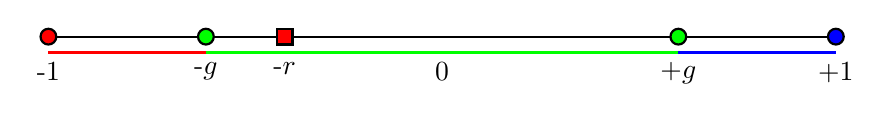
\begin{tikzpicture} [scale = 1] 
\draw[thick] (-5.0, 0.0) -- (5.0, 0.0);
\draw[fill = red, thick] (-5.0, 0.0) circle [radius = 0.1];
\draw[fill = green, thick] (-3.0, 0.0) circle [radius = 0.1];
\draw[fill = red, thick] (-2.1, -0.1) rectangle (-1.9, 0.1);
\draw[fill = green, thick] (3.0, 0.0) circle [radius = 0.1];
\draw[fill = blue, thick] (5.0, 0.0) circle [radius = 0.1];
\draw[red, thick] (-5.0, -0.2) -- (-3.0, -0.2);
\draw[green, thick] (-3.0, -0.2) -- (3.0, -0.2);
\draw[blue, thick] (3.0, -0.2) -- (5.0, -0.2);
\node[below] at (-5.0, -0.2){-$1$};
\node[below] at (-3.0, -0.2){-$g $};
\node[below] at (-2.0, -0.2){-$r $};
\node[below] at (0.0, -0.2){$0$};
\node[below] at (3.0, -0.2){+$g $};
\node[below] at (5.0, -0.2){+$1$};
\end{tikzpicture} \captionof{figure}{$1D$ Artificial Incentive-incompatible Example $1$ (Truthful)}\label{fig:1dat}
\end{figure}

\begin{figure}[H] \centering 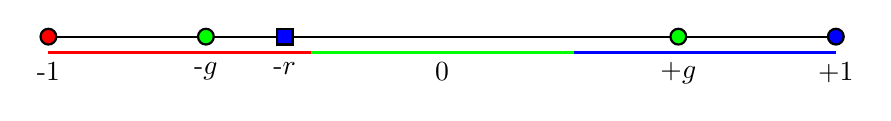
\begin{tikzpicture} [scale = 1] 
\draw[thick] (-5.0, 0.0) -- (5.0, 0.0);
\draw[fill = red, thick] (-5.0, 0.0) circle [radius = 0.1];
\draw[fill = green, thick] (-3.0, 0.0) circle [radius = 0.1];
\draw[fill = blue, thick] (-2.1, -0.1) rectangle (-1.9, 0.1);
\draw[fill = green, thick] (3.0, 0.0) circle [radius = 0.1];
\draw[fill = blue, thick] (5.0, 0.0) circle [radius = 0.1];
\draw[red, thick] (-5.0, -0.2) -- (-1.67, -0.2);
\draw[green, thick] (-1.67, -0.2) -- (1.67, -0.2);
\draw[blue, thick] (1.67, -0.2) -- (5.0, -0.2);
\node[below] at (-5.0, -0.2){-$1$};
\node[below] at (-3.0, -0.2){-$g $};
\node[below] at (-2.0, -0.2){-$r $};
\node[below] at (0.0, -0.2){$0$};
\node[below] at (3.0, -0.2){+$g $};
\node[below] at (5.0, -0.2){+$1$};
\end{tikzpicture} \captionof{figure}{$1D$ Artificial Incentive-incompatible Example $1$ (Misreport)}\label{fig:1dam}
\end{figure}
 Consider a 3-way classifier $h_t: \R \to  \left\{\text{\;red\;}, \text{\;green\;}, \text{\;blue\;}\right\} $ parametrized by $t\ge 0$:
 \begin{equation}
 h_{t}\left(x\right) =\left\{ \begin{array}{ll}
 \text{\;red\;}& \text{\;if\;} x < t  \\
 \text{\;green\;}& \text{\;if\;} -t \leq  x \leq  t \\
 \text{\;blue\;}& \text{\;if\;} x  > t. \\
 \end{array}\right. 
 \end{equation}
 Let the hypothesis space be
 \begin{equation}
 \H = \left\{ h_t : t \geq  0\right\}.
 \end{equation}
 Equivalently, a hypothesis $h_t$ partitions $\R$ into three sets: 
 $X^\text{red}_t = (-\infty, -t)$,
 $X^\text{green}_t = [-t, t]$,
 $X^\text{blue}_t = (t, \infty)$.
 Given a labeled point $(x,y)$ with  $y \in \left\{\text{\;red\;}, \text{\;green\;}, \text{\;blue\;}\right\}$, it could be outside the ``color region'' suggested by $h_t$. 
 Accordingly, we define a loss function $\ell$ based on the distance it takes to move the point to the corresponding color region suggested by $h_t$.
 Concretely,
 \begin{equation}
 \ell\left(x, y, h_t\right) = f(d(x, X^y_t))
 \end{equation}
 where 
 \begin{equation}
 d(x, X^y_t) = \min_{x' \in X^y_t} \|x-x'\|
 \end{equation}
 is the shortest distance from the point $x$ to the set (color region) $X^y_t$.
 $f \ge 0$ is strictly convex with minimum at 0: $f(0) = 0$.
 For example, $f$ can be the square function $f(z)=z^2$.
 
 Given a training set $S=\{(x_1,y_1), \ldots (x_n, y_n)\}$, consider the Empiricial Risk Minimizer (ERM)
 \begin{equation}
 \hat h \in \argmin_{h \in \H} \sum_{i=1}^n \ell(x_i, y_i, h).
 \end{equation}

We now exhibit a family of IIC datasets $S $ parameterized by $g $ and $r $, see Figure \ref{fig:1dat}. $S $ consists of five labeled points:
\begin{align*}
S\left(g, r\right)  &= \left\{\left(x_{i}, y_{i}\right)\right\}_{i=1}^{5} = \left\{\left(-1, \text{\;red\;}\right), \left(-g, \text{\;green\;}\right), \left(-r, \text{\;red\;}\right), \left(g, \text{\;green\;}\right), \left(1, \text{\;blue\;}\right)\right\},
\end{align*}
with $0 < r < g < 1$.
\newline \newline
\begin{prop} \label{prop:ex1} 
For any $g $, there exists an $r  \in \left(0, g\right)$ such that the dataset $S\left(g, r \right) $ is incentive incompatible with respect to ERM on $\mathcal{H}$ and $\ell$.
\end{prop}
\begin{proof} \label{proof:ex1pf} 
The optimal threshold for the original dataset is,
\[ t^\star  = \arg\displaystyle\min_{t \geq  0}\left\{ \begin{array}{ll}
f(t - r)& \text{\;if\;} t \geq  g \\
2 f\left(g - t\right) + f\left(t - r\right)& \text{\;if\;} r < t < g \\
2 f\left(g - t\right)& \text{\;if\;} t \leq  r \\
\end{array},\right. \]
Since $f\left(0\right)  = 0$, the objective is continuous at $t  = g $ and $t  = r $. Note that $f\left(t - r\right) $ is minimized at $r  < g$ and $f\left(t - g\right) $ is minimized at $g  > r$, we have,
\begin{align*}
&t^\star  \in \left(r , g \right),
\end{align*}
which classifies (-$r , \text{\;red\;}$) incorrectly as a green point.
\\* Similarly, the optimal threshold if the agent misreports her label as blue is,
\[ t^\star  = \arg\displaystyle\min_{t \geq  0}\left\{ \begin{array}{ll}
f(t + r)& \text{\;if\;} t \geq  g \\
2 f\left(g - t\right) + f\left(t + r\right)& \text{\;if\;} r \leq  t < g \\
2 f\left(g - t\right) + f\left(t + r\right)& \text{\;if\;} t < r \\
\end{array},\right. \]
Since $f\left(t + r\right) $ is minimized at $t  = -r < g $ and $f\left(g - t\right) $ is minimized at $g, $
\begin{align*}
&t^\star  \in \left(0, g \right),
\end{align*}
and the objective in this range is,
\begin{align*}
&2 f\left(g - t\right) + f\left(t + r\right).
\end{align*}
Define $\delta := g$ - r. Fix small $\varepsilon > 0$, there is sufficiently small $\delta > 0$ such that, due to strict convexity,
\begin{align*}
2 \dfrac{f\left(\delta + \varepsilon\right) - f\left(\delta\right)}{\varepsilon} &< \dfrac{f\left(2 r\right) - f\left(2 r - \varepsilon\right)}{\varepsilon} .
\end{align*}
This inequality implies that the objective at $t  = r  - \varepsilon$,
\begin{align*}
2 f\left(\delta + \varepsilon\right) + f\left(2 r - \varepsilon\right) &< 2 f\left(\delta\right) + f\left(2 r \right),
\end{align*}
which is the objective at $t  = r $. Therefore, the objective is decreasing at $r $, given that it is the sum of two strictly convex functions thus strictly convex itself, we have,
\begin{align*}
&t^\star  \in \left(0, r \right),
\end{align*}
which classifies (-$r , \text{\;red\;}$) correctly as a red point.
\\* Therefore, the point has the incentive to misreport and the dataset is incentive incompatible.
\newline \newline\end{proof}
\begin{eg} \label{eg:ex1sq} 
When $f $ is differentiable, there is a sufficient (but not necessary) condition on $g $ and $r $ such that $S\left(g, r \right) $ is IIC,
\begin{align*}
2 f'\left(g - r\right) &< f'\left(2 r\right).
\end{align*}
For any strictly convex $f $ satisfying $f\left(0\right)  = 0$ and $f'\left(0\right)  = 0$, for any fixed $g $, there exists at least one $r $ that satisfies the above condition since $f'\left(2 r\right)  > 0$ and $\lim_{g \to  r^{+}} f'\left(g - r\right) \to  f'\left(0\right) = 0$.
\\* When the condition holds, the objective at $t  = r $ is increasing, implying that $t^\star $ is less than $r $, and the corresponding classifier classifies (-$r , \text{\;red\;}$) correctly as a red point when the agent misreports her label as blue.
\newline \newline\end{eg}
\begin{eg} \label{eg:ex2sq} 
When $f $ is the square function, the loss is the square of the distance it takes to move the point to the correct region. In this case, $S\left(g, r\right) $ is IIC as long as $g  < 2 r. $
\\* In particular, the optimal threshold for the original dataset is,
\begin{align*}
t^\star  &= \dfrac{2}{3} g + \dfrac{1}{3} r \in \left(r , g \right),
\end{align*}
which classifies (-$r , \text{\;red\;}$) incorrectly as a green point, but the optimal threshold if the agent misreports her label as blue is,
\begin{align*}
t^\star  &= \dfrac{2}{3} g - \dfrac{1}{3} r \in \left(0, r \right),
\end{align*}
which classifies (-$r , \text{\;red\;}$) correctly as a red point.
\newline \newline\end{eg}


\subsection{Another Example}

Intuitively, when the misclassified class-$1$ point pretends to be a class-$3$ point with a large loss, the classifier modifies the $2$-vs-$3$ decision boundary to minimize that loss, and the point benefits from the interdependence between the $2$-vs-$3$ decision and the $1$-vs-$2$ decision.
\newline \newline
The decision boundaries can be related in more complicated ways. Consider the three-class $1D$ threshold classifiers in the form,
\[ \hat{y}\left(x; l\right) =\left\{ \begin{array}{ll}
1& \text{\;if\;} x < l \\
2& \text{\;if\;} l \leq  x \leq  r \\
3& \text{\;if\;} x > r \\
\end{array}\right. \]
This is effectively a one-vs-one threshold classifier with the $1$-vs-$2$ threshold of $l $, with the $2$-vs-$3$ threshold of $r $ and the $1$-vs-$3$ threshold of any value between $l $ and $r $. Now define the loss function as the squared distance to the center of the decision region (bounded by the range of the data),
\[ \ell\left(x_{i}, y_{i}; t\right) =\left\{ \begin{array}{ll}
\left(x_{i} - \dfrac{l + \displaystyle\min_{i} x_{i}}{2}\right)^{2}& \text{\;if\;} y_{i} = 1 \\
\left(x_{i} - \dfrac{l + r}{2}\right)^{2}& \text{\;if\;} y_{i} = 2 \\
\left(x_{i} - \dfrac{r + \displaystyle\max_{i} x_{i}}{2}\right)^{2}& \text{\;if\;} y_{i} = 3 \\
\end{array}\right. \]
Then, the learner's maximization problem is,
\begin{align*}
&\displaystyle\min_{t \in \mathbb{R}} \ell\left(x_{i}, y_{i}; t\right).
\end{align*}
The agent's problem is to minimize the loss for their point with their true label. The loss can be either the distance-to-center loss or zero-one loss, here, for simplicity, assume the agents also want to minimize the distance to the center,
\begin{align*}
&\displaystyle\max_{y^{\dagger}_{i} \in \left\{1, 2, 3\right\}} \ell\left(x_{i}, y_{i}; l^\star \left(y^{\dagger}_{i}\right), r^\star \left(y^{\dagger}_{i}\right)\right),
\end{align*}
where $l^\star \left(y^{\dagger}_{i}\right)$ and $r^\star \left(y^{\dagger}_{i}\right)$ are the optimal thresholds for the learner when agent $i $ misreports the label as $y^{\dagger}_{i.}$
\\* For the same dataset $\left\{\left(x_{i}, y_{i}\right)\right\}_{i=1}^{5} = \left\{\left(-5, 1\right), \left(-3, 2\right), \left(-2, 1\right), \left(4, 2\right), \left(5, 3\right)\right\}$, the minimum loss is $29.5$ and it occurs when $l  = -2.5$ and $r = 4$ when every agent reports truthfully. In this case, agent (-$2, 1$) is misclassified as (-$2, 2$). However, if (-$2, 1$) misreports as (-$2, 3$), the loss from $l  = -2.5$ and $r = 4$ is above $68$ and the minimum loss is $57$ and it occurs when $l  = -1$ and $r  = 0$. In this case, agent (-$2, 1$) is classified correctly. In particular, the agent (-$2, 1$) improves the loss from $1$ to $0$.
\newline \newline

\begin{figure}[H] \centering 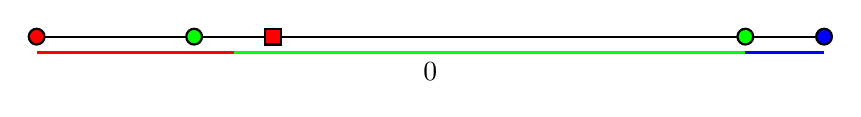
\begin{tikzpicture} [scale = 1] 
\draw[thick] (-5.0, 0.0) -- (5.0, 0.0);
\draw[fill = red, thick] (-5.0, 0.0) circle [radius = 0.1];
\draw[fill = green, thick] (-3.0, 0.0) circle [radius = 0.1];
\draw[fill = red, thick] (-2.1, -0.1) rectangle (-1.9, 0.1);
\draw[fill = green, thick] (4.0, 0.0) circle [radius = 0.1];
\draw[fill = blue, thick] (5.0, 0.0) circle [radius = 0.1];
\draw[red, thick] (-5.0, -0.2) -- (-2.5, -0.2);
\draw[green, thick] (-2.5, -0.2) -- (4.0, -0.2);
\draw[blue, thick] (4.0, -0.2) -- (5.0, -0.2);
\node[below] at (0.0, -0.2){$0$};
\end{tikzpicture} \captionof{figure}{$1D$ Artificial Incentive-incompatible Example $2$ (Truthful)}\label{fig:2dat}
\end{figure}

\begin{figure}[H] \centering 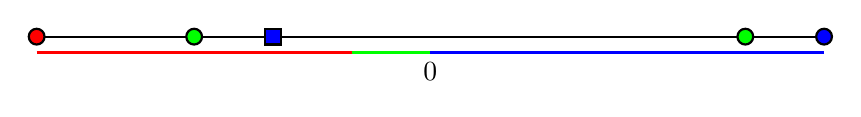
\begin{tikzpicture} [scale = 1] 
\draw[thick] (-5.0, 0.0) -- (5.0, 0.0);
\draw[fill = red, thick] (-5.0, 0.0) circle [radius = 0.1];
\draw[fill = green, thick] (-3.0, 0.0) circle [radius = 0.1];
\draw[fill = blue, thick] (-2.1, -0.1) rectangle (-1.9, 0.1);
\draw[fill = green, thick] (4.0, 0.0) circle [radius = 0.1];
\draw[fill = blue, thick] (5.0, 0.0) circle [radius = 0.1];
\draw[red, thick] (-5.0, -0.2) -- (-1.0, -0.2);
\draw[green, thick] (-1.0, -0.2) -- (0.0, -0.2);
\draw[blue, thick] (0.0, -0.2) -- (5.0, -0.2);
\node[below] at (0.0, -0.2){$0$};
\end{tikzpicture} \captionof{figure}{$1D$ Artificial Incentive-incompatible Example $2$ (Misreport)}\label{fig:2dam}
\end{figure}
To generalize the above observations, suppose the learner is a probabilistic classifier with parameters estimated by maximum likelihood, and the agents report their labels to maximize the classification probability of their true labels. Then the following two conditions guarantee that the classification is incentive-compatible.
\newline \newline
\begin{df} \label{df:mono} 
(Monotonic Condition) A multi-class probabilistic classifier is monotonic if, given a training set $S $, for any point $x $ with labels $a $ and $b, $
\begin{align*}
\dfrac{\mathbb{P}\left\{Y = a | x ; w^\star \left(S\right)\right\}}{\mathbb{P}\left\{Y = b | x ; w^\star \left(S\right)\right\}} &\geq  \dfrac{\mathbb{P}\left\{Y = a | x ; w^\star \left(S \cup \left\{\left(x, y = a\right)\right\}\right)\right\}}{\mathbb{P}\left\{Y = b | x ; w^\star \left(S \cup \left\{\left(x, y = a\right)\right\}\right)\right\}}.
\end{align*}\end{df}
The assumption says that the probability that $x $ is classified as $a $ increases when there is an additional point $\left(x , a \right)$ in the training set.
\newline \newline
\begin{df} \label{df:iia} 
(Independence of Irrelevant Alternatives (IIA) Condition) A multi-class classifier is independent of irrelevant alternatives if, given a training set $S $, for any point $x $ and any pair of labels $a $ and $b, $
\begin{align*}
\dfrac{\mathbb{P}\left\{Y = a | x ; w^\star \left(S\right)\right\}}{\mathbb{P}\left\{Y = b | x ; w^\star \left(S\right)\right\}} &= \dfrac{\mathbb{P}\left\{Y = a | x ; w^\star \left(S \cup \left\{\left(x', y' \notin \left\{a, b\right\}\right)\right\}\right)\right\}}{\mathbb{P}\left\{Y = b | x ; w^\star \left(S \cup \left\{\left(x', y' \notin \left\{a, b\right\}\right)\right\}\right)\right\}}.
\end{align*}\end{df}
The assumption says that the ratio between the classification probabilities of $x $ of any two classes is not changed by adding a point at $x $ with a third class.
\newline \newline
Combining the two assumptions MC and IIA, we have that an agent with label $a $ cannot change the decision of $a $ vs $b $ by misreporting its label as a third class $c $. This observation is formalized in the following proposition.
\newline \newline
\begin{thm} \label{thm:margin} 
A multi-class probabilistic classifier estimated by maximum likelihood is incentive-compatible if it is monotonic and independent of irrelevant alternatives.
\end{thm}
\begin{proof} \label{proof:marginpf} 
Fix a dataset $\left\{\left(x_{i}, y_{i}\right)\right\}_{i=1}^{n}$, let the maximum likelihood estimates in the case every agent report truthfully be,
\begin{align*}
w^\star  &= \arg\displaystyle\max_{w} \displaystyle\sum_{i'=1}^{n} \log\left(\mathbb{P}\left\{Y = y_{i'} | x_{i'} ; w\right\}\right).
\end{align*}
Fix an agent $i $, her feature vector $x_{i}$, and fix other agents' reports, $\left(x_{-i}, y_{-i}\right)$, define the maximum likelihood estimate given the misreport of agent $i , y^{\dagger}_{i}$ as,
\begin{align*}
w^{\dagger} &= \arg\displaystyle\max_{w} \displaystyle\sum_{i'=1, i' \neq  i}^{n} \log\left(\mathbb{P}\left\{Y = y_{i'} | x_{i'}, w\right\}\right) + \log\left(\mathbb{P}\left\{Y = y^{\dagger}_{i} | x_{i} ; w\right\}\right).
\end{align*}
Now suppose, for a contradiction, that agent $i $ prefers misreporting, assume the following incentive inequality,
\begin{align*}
\mathbb{P}\left\{Y = y_{i} | x_{i} ; w^\star \right\} &> \mathbb{P}\left\{Y = y_{i} | x_{i} ; w^{\dagger}\right\}.
\end{align*}
If there are only two classes, then by symmetry,
\begin{align*}
\mathbb{P}\left\{Y = y^{\dagger}_{i} | x_{i} ; w^\star \right\} &< \mathbb{P}\left\{Y = y^{\dagger}_{i} | x_{i} ; w^{\dagger}\right\}.
\end{align*}
If there are more than two classes, fix a third $y'_{i} \notin \left\{y_{i}, y^{\dagger}_{i}\right\}$, and define an intermediate maximum likelihood estimate from removing the point $\left(x_{i}, y_{i}\right)$,
\begin{align*}
w' &= \arg\displaystyle\max_{w} \displaystyle\sum_{i'=1, i' \neq  i}^{n} \log\left(\mathbb{P}\left\{Y = y_{i'} | x_{i'} ; w\right\}\right),
\end{align*}
then the Monotonic Condition implies,
\begin{align*}
\dfrac{\mathbb{P}\left\{Y = y_{i} | x_{i} ; w^\star \right\}}{\mathbb{P}\left\{Y = y'_{i} | x_{i} ; w^\star \right\}} &\leq  \dfrac{\mathbb{P}\left\{Y = y_{i} | x_{i} ; w'\right\}}{\mathbb{P}\left\{Y = y'_{i} | x_{i} ; w'\right\}},
\end{align*}
and the IIA Condition implies,
\begin{align*}
\dfrac{\mathbb{P}\left\{Y = y_{i} | x_{i} ; w'\right\}}{\mathbb{P}\left\{Y = y'_{i} | x_{i} ; w'\right\}} &= \dfrac{\mathbb{P}\left\{Y = y_{i} | x_{i} ; w^{\dagger}\right\}}{\mathbb{P}\left\{Y = y'_{i} | x_{i} ; w^{\dagger}\right\}}.
\end{align*}
Combining the above two inequalities with the incentive inequality, we have,
\begin{align*}
\mathbb{P}\left\{Y = y'_{i} | x_{i} ; w^\star \right\} &> \mathbb{P}\left\{Y = y'_{i} | x_{i} ; w^{\dagger}\right\}.
\end{align*}
Note that the above inequality is true for all $y'_{i} \notin \left\{y_{i}, y^{\dagger}_{i}\right\}$, summing over all such $y'_{i}$ results in,
\begin{align*}
\displaystyle\sum_{y \notin \left\{y_{i}, y^{\dagger}_{i}\right\}} \mathbb{P}\left\{Y = y'_{i} | x_{i} ; w^\star \right\} &> \displaystyle\sum_{y \notin \left\{y_{i}, y^{\dagger}_{i}\right\}} \mathbb{P}\left\{Y = y'_{i} | x_{i} ; w^{\dagger}\right\},
\end{align*}
given that the class probabilities sum up to $1$,
\begin{align*}
1 - \mathbb{P}\left\{Y = y_{i} | x_{i} ; w^\star \right\} - \mathbb{P}\left\{Y = y^{\dagger}_{i} | x_{i} ; w^\star \right\} &> 1 - \mathbb{P}\left\{Y = y_{i} | x_{i} ; w^{\dagger}\right\} - \mathbb{P}\left\{Y = y^{\dagger}_{i} | x_{i} ; w^{\dagger}\right\},
\end{align*}
and using the incentive inequality again,
\begin{align*}
\mathbb{P}\left\{Y = y^{\dagger}_{i} | x_{i} ; w^\star \right\} &< \mathbb{P}\left\{Y = y^{\dagger}_{i} | x_{i} ; w^{\dagger}\right\}.
\end{align*}
Now, due to the optimality of $h^{\dagger,}$
\begin{align*}
&  \displaystyle\sum_{i'=1, i' \neq  i}^{n} \log\left(\mathbb{P}\left\{Y = y_{i'} | x_{i'} ; w^{\dagger}\right\}\right) + \log\left(\mathbb{P}\left\{Y = y^{\dagger}_{i} | x_{i} ; w^{\dagger}\right\}\right)
\\ &\leq  \displaystyle\sum_{i'=1, i' \neq  i}^{n} \log\left(\mathbb{P}\left\{Y = y_{i'} | x_{i'} ; w^\star \right\}\right) + \log\left(\mathbb{P}\left\{Y = y^{\dagger}_{i} | x_{i} ; w^\star \right\}\right),
\end{align*}
using the above inequalities, the comparison can be simplified to,
\begin{align*}
\displaystyle\sum_{i'=1, i' \neq  i}^{n} \log\left(\mathbb{P}\left\{Y = y_{i'} | x_{i'} ; w^{\dagger}\right\}\right) &< \displaystyle\sum_{i'=1, i' \neq  i}^{n} \log\left(\mathbb{P}\left\{Y = y_{i'} | x_{i'} ; w^\star \right\}\right),
\\ \displaystyle\sum_{i'=1}^{n} \log\left(\mathbb{P}\left\{Y = y_{i'} | x_{i'} ; w^{\dagger}\right\}\right) &< \displaystyle\sum_{i'=1}^{n} \log\left(\mathbb{P}\left\{Y = y_{i'} | x_{i'} ; w^\star \right\}\right),
\end{align*}
which is a contradiction to the optimality of $w^\star $.
\newline \newline\end{proof}
\begin{cor} \label{cor:binpr} 
Binary probabilistic classifiers estimated by maximum likelihood are incentive-compatible.
\end{cor}
\begin{proof} \label{proof:binpr} 
MC holds due to the optimality conditions and IIA holds since there are only two classes.
\newline \newline\end{proof}
The assumptions Definition \ref{df:mono} (MC) and Definition \ref{df:iia} (IIA) can be significantly simplified for a separable class of the classifiers.
\newline \newline
\begin{df} \label{df:sep} 
A probabilistic classifier is separable if the parameters $w^\star $ can be partitioned into $k $ classes, $w^\star _{1}, w^\star _{2}, ..., w^\star _{k}$, one set of parameters for each class, such that for given training sets $S $ and $S'$ and any label $a $ if,
\begin{align*}
\left\{\left(x_{i}, y_{i}\right) \in S : y_{i} = a\right\} &= \left\{\left(x_{i}, y_{i}\right) \in S' : y_{i} = a\right\},
\end{align*}
then,
\begin{align*}
w^\star _{a}\left(S\right) &= w^\star _{a}\left(S'\right),
\end{align*}
and if there is a value function $v_{a}\left(x; w^\star _{a}\right)$ that are independent of $w^\star _{b}, b \neq  a $ such that,
\begin{align*}
\mathbb{P}\left\{Y = y | x; w^\star \right\} &= \dfrac{v_{a}\left(x; w^\star _{a}\right)}{\displaystyle\sum_{b=1}^{K} v_{b}\left(x; w^\star _{b}\right)},
\end{align*}
then the classifier is separable.
\newline \newline\end{df}
Logistic regression satisfies the value function requirement but fails the separability condition since training $w^\star _{a}$ uses data with labels that are not $a $. On the other hand, Bayes-type classifiers are separable. For separable classifiers, Definition \ref{df:mono} (MC) and Definition \ref{df:iia} (IIA) are always satisfied.
\newline \newline
\begin{cor} \label{cor:sepmargin} 
A separable multi-class probabilistic classifier estimated by maximum likelihood is incentive-compatible.
\end{cor}
\begin{proof} \label{proof:sepmarginpf} 
Due to separability,
\begin{align*}
v_{a}\left(x; w^\star \left(S\right)\right) &= v_{a}\left(x; w^\star \left(S \cup \left\{\left(x', y' \notin \left\{a, b\right\}\right)\right\}\right)\right), \text{\;and\;}
\\ v_{b}\left(x; w^\star \left(S\right)\right) &= v_{b}\left(x; w^\star \left(S \cup \left\{\left(x, y = a\right)\right\}\right)\right) = v_{b}\left(x; w^\star \left(S \cup \left\{\left(x', y' \notin \left\{a, b\right\}\right)\right\}\right)\right).
\end{align*}
MC follows from the optimality condition of $w^\star \left(S\right)$ and IIA follows immediately.
\newline \newline\end{proof}
\begin{cor} \label{cor:bc} 
Bayes classifiers estimated by maximum likelihood are incentive-compatible.
\end{cor}
\begin{proof} \label{proof:bcpf} 
Follows from Corollary \ref{cor:sepmargin}.
\newline \newline\end{proof}
Kernel density estimators are not estimated by maximum likelihood, so the previous results do not hold, although the proof is similar. There are two general approaches to use kernel densities for classification, the first is to use all the points to estimate the density and the second is to estimate the densities for each class separately (see \citet*{taylor1997classification}). The second approach is similar to a separable classifier. K-Nearest Neighbor is a special case of this with a uniform kernel.
\newline \newline
\begin{cor} \label{cor:kde} 
Kernel density estimators are incentive-compatible.
\end{cor}
\begin{proof} \label{proof:kdepf} 
The first approach suggests that,
\begin{align*}
\mathbb{P}\left\{X = x\right\} &= \dfrac{1}{n h^{D}} \displaystyle\sum_{i'=1}^{n} w_{i'}, \text{\;where\;} w_{i'} = K\left(\dfrac{x - x_{i'}}{h}\right).
\end{align*}
Define $w^\star $ as the weight function when all agents report truthfully, and $w^{\dagger} = w^\star \left(y^{\dagger}_{i}\right)$ as the weight if agent $i $ misreports, then the classification probabilities for agent $i $ from dividing up the sum based on the class is,
\begin{align*}
\mathbb{P}\left\{Y = y_{i} | x_{i} ; w^\star \right\} &= \dfrac{1}{n} \displaystyle\sum_{i'=1}^{n} w^\star _{i'} \mathbbm{1}_{\hat{y}_{i'} = y_{i}}
\\ &= \dfrac{1}{n} \displaystyle\sum_{i'=1}^{n} w^\star _{i'} \mathbbm{1}_{\hat{y}_{i'} = y_{i}, i' \neq  i} + \dfrac{1}{n} w^\star _{i}
\\ &= \mathbb{P}\left\{Y = y_{i} | x_{i} ; w^{\dagger}\right\} + \dfrac{1}{n} K\left(0\right), \text{\;since\;} y^{\dagger}_{i} \neq  y_{i}
\\ &\leq  \mathbb{P}\left\{Y = y_{i} | x = x_{i} ; w^\star \dagger\right\},
\end{align*}
meaning reporting truthfully results in a larger probability compared to reporting $y^{\dagger}_{i}$ instead.
\\* Alternatively, the second approach suggests that, if the classification probabilities are computed based on \citet*{taylor1997classification},
\begin{align*}
\mathbb{P}\left\{X = x | Y = y\right\} &= \dfrac{1}{n_{y} h^{D}} \displaystyle\sum_{i'=1}^{n} w_{i'} \mathbbm{1}_{\hat{y}_{i'} = y}, n_{y} = \displaystyle\sum_{i'=1}^{n} \mathbbm{1}_{\hat{y}_{i'} = y}
\end{align*}
Similar to the above derivation (and also as a special case of a Bayes estimator),
\begin{align*}
\mathbb{P}\left\{Y = y_{i} | x_{i} ; w^\star \right\} &= \dfrac{1}{n_{y}} \displaystyle\sum_{i'=1}^{n} w^\star _{i'} \mathbbm{1}_{\hat{y}_{i'} = y_{i}}
\\ &= \mathbb{P}\left\{Y = y_{i} | x_{i} ; w^\star \dagger\right\} + \dfrac{1}{n_{y}} K\left(0\right)
\\ &\leq  \mathbb{P}\left\{Y = y_{i} | x_{i} ; w^\star \dagger\right\}.
\end{align*}\end{proof}


\subsection{Empirical Risk Minimization}
A similar result can be obtained for empirical risk minimization. We could either add an assumption that the loss function can be normalized so that the sum is constant and it behaves the same way as a probabilistic classifier, or we could use stronger Monotonic and IIA Conditions. Here, we state the additional normalization condition.
\newline \newline
\begin{df} \label{df:nrml} 
(Normalized Loss) A loss function $\ell$ is normalized if given a hypothesis $h $, for any point,
\begin{align*}
\displaystyle\sum_{y} \ell\left(y ; h\right) &= C , \text{\;constant\;} .
\end{align*}\end{df}
\begin{df} \label{df:monoerm} 
(Monotonic Condition for ERM) Multi-class empirical risk minimization classifiers are monotonic if, given a training set $S $, for any point $x $ with labels $a $ and $b, $
\begin{align*}
\dfrac{\ell\left(y = a ; h^\star \left(S\right)\right)}{\ell\left(y = b ; h^\star \left(S\right)\right)} &\geq  \dfrac{\ell\left(y = a ; h^\star \left(S \cup \left\{\left(x, y = a\right)\right\}\right)\right)}{\ell\left(y = b ; h^\star \left(S \cup \left\{\left(x, y = a\right)\right\}\right)\right)}.
\end{align*}\end{df}
\begin{df} \label{df:iiaerm} 
(IIA Condition for ERM) Multi-class empirical risk minimization classifiers are independent of irrelevant alternatives if, given a training set $S $, for any point $x $ and any pair of labels $a $ and $b, $
\begin{align*}
\dfrac{\ell\left(y = a ; h^\star \left(S\right)\right)}{\ell\left(y = b ; h^\star \left(S\right)\right)} &= \dfrac{\ell\left(y = a ; h^\star \left(S \cup \left\{\left(x', y' \notin \left\{a, b\right\}\right)\right\}\right)\right)}{\ell\left(y = b ; h^\star \left(S \cup \left\{\left(x', y' \notin \left\{a, b\right\}\right)\right\}\right)\right)}.
\end{align*}\end{df}
\begin{cor} \label{cor:marginerm} 
Multi-class empirical risk minimization classifiers with normalized loss functions are incentive-compatible if it is monotonic and independent of irrelevant alternatives.
\end{cor}
\begin{proof} \label{proof:marginermpf} 
For a fixed dataset $\left\{\left(x_{i}, y_{i}\right)\right\}_{i=1}^{n}$, and the hypothesis class $\mathcal{H}$, let the optimal classifier in the case every agent report truthfully be,
\begin{align*}
h^\star  &= \arg\displaystyle\min_{h \in \mathcal{H}} \displaystyle\sum_{i'=1}^{n} \ell\left(y_{i'} ; h\right).
\end{align*}
Fix an agent $i $, her feature vector $x_{i}$, and fix other agents' reports, $\left(x_{-i}, y_{-i}\right)$, define the optimal classifier given the classifier $h $ and the misreport of agent $i , y^{\dagger}_{i}$ as,
\begin{align*}
h^{\dagger} &= \arg\displaystyle\min_{h \in \mathcal{H}} \displaystyle\sum_{i'=1, i' \neq  i}^{n} \ell\left(y_{i'} ; h\right) + \ell\left(y^{\dagger}_{i} ; h\right).
\end{align*}
Now suppose, for a contradiction, that agent $i $ prefers misreporting, assume the following incentive inequality,
\begin{align*}
\ell\left(y_{i} ; h^\star \right) &> \ell\left(y_{i} ; h^{\dagger}\right).
\end{align*}
If there are only two classes, then by symmetry,
\begin{align*}
\ell\left(y^{\dagger}_{i} ; h^\star \right) &< \ell\left(y^{\dagger}_{i} ; h^{\dagger}\right).
\end{align*}
If there are more than two classes, fix a third $y'_{i} \notin \left\{y_{i}, y^{\dagger}_{i}\right\}$, and define an intermediate maximum likelihood estimate from removing the point $\left(x_{i}, y_{i}\right)$,
\begin{align*}
h' &= \arg\displaystyle\min_{h \in \mathcal{H}} \displaystyle\sum_{i' = 1, i' \neq  i}^{n} \ell\left(y_{i'} ; h\right),
\end{align*}
then the Monotonic Condition for ERM implies,
\begin{align*}
\dfrac{\ell\left(y_{i} ; h^\star \right)}{\ell\left(y'_{i} ; h^\star \right)} &\leq  \dfrac{\ell\left(y_{i} ; h'\right)}{\ell\left(y'_{i} ; h'\right)},
\end{align*}
and the IIA Condition implies,
\begin{align*}
\dfrac{\ell\left(y_{i} ; h'\right)}{\ell\left(y'_{i} ; h'\right)} &= \dfrac{\ell\left(y_{i} ; h^{\dagger}\right)}{\ell\left(y'_{i} ; h^{\dagger}\right)}.
\end{align*}
Combining the above two inequalities with the incentive inequality, we have,
\begin{align*}
\ell\left(y'_{i} ; h^\star \right) &> \ell\left(y'_{i} ; h^{\dagger}\right).
\end{align*}
Note that the above inequality is true for all $y'_{i} \notin \left\{y_{i}, y^{\dagger}_{i}\right\}$, summing over all such $y'_{i}$ results in,
\begin{align*}
\displaystyle\sum_{y \notin \left\{y_{i}, y^{\dagger}_{i}\right\}} \ell\left(y'_{i} ; h^\star \right) &> \displaystyle\sum_{y \notin \left\{y_{i}, y^{\dagger}_{i}\right\}} \ell\left(y'_{i} ; h^{\dagger}\right),
\end{align*}
and given the losses are normalized,
\begin{align*}
C  - \ell\left(y_{i} ; h^\star \right) - \ell\left(y^{\dagger}_{i} ; h^\star \right) &> C  - \ell\left(y_{i} ; h^{\dagger}\right) - \ell\left(y^{\dagger}_{i} ; h^{\dagger}\right),
\end{align*}
and using the incentive inequality again,
\begin{align*}
\ell\left(y^{\dagger}_{i} ; h^\star \right) &< \ell\left(y^{\dagger}_{i} ; h^{\dagger}\right).
\end{align*}
Now, due to the optimality of $h^{\dagger,}$
\begin{align*}
\displaystyle\sum_{i'=1, i' \neq  i}^{n} \ell\left(y_{i'} ; h^{\dagger}\right) + \ell\left(y^{\dagger}_{i} ; h^{\dagger}\right) &\leq  \displaystyle\sum_{i'=1, i' \neq  i}^{n} \ell\left(y_{i'} ; h^\star \right) + \ell\left(y^{\dagger}_{i} ; h^\star \right),
\end{align*}
using the above inequalities, the comparison can be simplified to,
\begin{align*}
\displaystyle\sum_{i'=1, i' \neq  i}^{n} \ell\left(y_{i'} ; h^{\dagger}\right) &\leq  \displaystyle\sum_{i'=1, i' \neq  i}^{n} \ell\left(y_{i'} ; h^\star \right),
\\ \displaystyle\sum_{i'=1}^{n} \ell\left(y_{i'} ; h^{\dagger}\right) &\leq  \displaystyle\sum_{i'=1}^{n} \ell\left(y_{i'} ; h^\star \right),
\end{align*}
which is a contradiction to the optimality of $h^\star $.
\newline \newline\end{proof}
\bibliographystyle{te}
\bibliography{cs}


\end{document}
